\documentclass[a4paper]{article}
\usepackage[a4paper,top=2cm,bottom=2cm,left=0.5cm,right=0.5cm,marginparwidth=1.75cm]{geometry}
\usepackage[]{graphicx}
\usepackage[]{wrapfig}
\usepackage[T2A]{fontenc}
\usepackage[utf8]{inputenc}
\usepackage[english, russian]{babel}
\usepackage[]{amsmath,amsfonts,amssymb,amsthm,mathtools}
\usepackage[]{wasysym}
\usepackage[]{float}
\usepackage{multicol}
\usepackage{mathtext}
\usepackage{amsmath}
\usepackage{amsfonts}
\usepackage{indentfirst}
\usepackage{longtable}
\usepackage{natbib}
\usepackage{mathrsfs}
\title{Исследование неизвестной на момент заголовка функции}
\date{\today}
\begin{document}
\maketitle
\section{Введение в проблему}
На операционном столе сегодня находится следующая функция:\\
$f(x) = sin(2*x^{2}+14)$\\
После некоторых очевиднейших преобразований получаем :\\
$f(x) = sin(2*x^{2}+14)$\\
\section{Нахождение первой производной}
Найдем $f\prime(x)$ :\\Очевидно, что:\\
$cos(2*x^{2}+14)*((2*x^{2})\prime+(14)\prime)$\\
У внимательного читателя возникнет вопрос: "почему так?" Не очень внимательный автор отчета даст такой ответ: "хз" и напишет:\\
$cos(2*x^{2}+14)*((2)\prime*x^{2}+2*(x^{2})\prime+(14)\prime)$\\
Имеем $f\prime(x) = cos(2*x^{2}+14)*2*2*x$\\
\section{Нахождение второй производной}
$f\prime\prime(x) = (cos(2*x^{2}+14)*2*2*x)\prime$\\ 
что?:\\
$(0-cos(2*x^{2}+14))*((2*x^{2}+14)\prime)*2*2*x+cos(2*x^{2}+14)*(2*2*x)\prime$\\
Ладно:\\
$(0-cos(2*x^{2}+14))*((2*x^{2})\prime+(14)\prime)*2*2*x+cos(2*x^{2}+14)*(2*2*x)\prime$\\
Если бы вы посещали вуз, вы бы знали, что:\\
$(0-cos(2*x^{2}+14))*((2)\prime*x^{2}+2*(x^{2})\prime+(14)\prime)*2*2*x+cos(2*x^{2}+14)*(2*2*x)\prime$\\
Автору не очень хочется писать, как он получил все это, поэтому он просто напишет "очевидным переходом получаем":\\
$(0-cos(2*x^{2}+14))*(0*x^{2}+2*2*x+0)*2*2*x+cos(2*x^{2}+14)*(0*2*x+2*((2)\prime*x+2*(x)\prime))$\\
Имеем $f\prime\prime(x) = (0-cos(2*x^{2}+14))*2*2*x*2*2*x+cos(2*x^{2}+14)*4$\\
\section{Найдем первую и вторую производную в точке, а также саму функцию}
$f(2) = -0.00885131$\\
$f\prime(2) = -7.99969 $\\
И вторую производную: \\ 
$f(2)\prime\prime = 59.9976$ \\
\section{График}
На данном графике в районе $\pm 10$ от заданной точки указаны: \\
Красный - сама функция \\
Зеленый - первая производная \\
Синий - вторая производная \\
\begin{figure}[H]
\centering
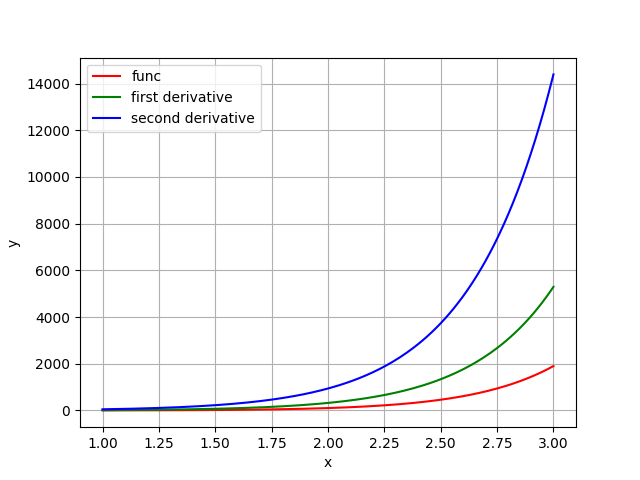
\includegraphics{graph.png}
\end{figure}\section{Тэйлор в точке до o($x^7$)}
Далее мы неиронично разложим функцию в ряд тэйлора в точке $x0 = 2$: \\
$f(x) = -0.00885131 + \frac{-7.99969}{1}(x-2)^{1} + \frac{59.9976}{2}(x-2)^{2} + \frac{-415.984}{6}(x-2)^{3} + \frac{2607.9}{24}(x-2)^{4} + \frac{-14207.4}{120}(x-2)^{5} + \frac{61501.6}{720}(x-2)^{6} + \frac{-151034}{5040}(x-2)^{7} + o(x^7)$
\end{document}